
\section{Generalized taxonomy based join
	
	
	}

We now turn to a general case when one string  matches multiple nodes in a taxonomy. Specifically, we first propose a generalized similarity function  which naturally extends the previous TS function, and then we show three attractive properties that this new function guarantees, and finally we study how to perform the efficient string join based on this function.



\subsection{Generalised similarity functions}

Given two strings, each of which can match multiple nodes in a
taxonomy, to measure the similarity between these two strings, we
extend the previous function by using maximum similarity matching in a bipartite
graph. Intuitively, see Figure , where each string contains multiple substring to match nodes in a taxonomy. And there is the similarity of two nodes in two strings can measure with TS function. Then the overall similarity can be naturally measured with the maximum similairty matching in a bipartite graph, formally defined as follows.   


\begin{figure}[t]
	\centering
	\includegraphics[scale=0.4]{figures/bipartite}
	\caption{Illustration to the maximum matching in bipartite graphs}
	\label{fig:bipartite}
\end{figure}

Based on the previous similarity function TS, we propose a new similarity function as follows:

\begin{definition} [Weight functions] Given two tokens (words) $s_i$ and $t_j$ and a taxonomy $\mathcal{T}$, the weight function $w$: $s_i \times t_j \rightarrow \mathcal{R} $ is defined by $w(s_i, t_j, \mathcal{T})$ = $TS(s_i, t_j, \mathcal{T})$.
\label{def:weightfunction}\end{definition}

\begin{definition} [Maximum Similarity Matching] Given a taxonomy $\mathcal{T}$ and two strings $s$ and $t$, for each tokens $s_i \in s$ and $t_j \in t$, there is a weight function $w$: $s_i \times t_j \rightarrow \mathcal{R}$. A maximum similarity matching  $M$ is defined as a matching where the sum of weight functions $w(s_i, t_j, \mathcal{T})$ for all distinct pairs ($s_i$, $t_j$) have a maximal value.  \label{def:maximum similaritymatching}
\end{definition}

\smallskip

Note that the distinct match means that all $s_i$ should be different in $s$, so this is similar to the maximum matching in a bipartite graph.

\smallskip


\begin{definition} [Generalised taxonomy similarity] Given two strings $s$ and $t$ and a taxonomy $\tau$, the similarity denoted by GTS($s$,$t$,$\tau$) =   $\frac{W(s,t,\tau)}{max(|s|,|t|)}$, where $W(s,t,\tau)$ is the weight of the maximum similarity matching $M$.  \label{def:efs}
\end{definition}

\smallskip

\begin{example} Consider two strings ``\textsf{Riverside California}'' and ``\textsf{Cupertino US}'', the maximal matching is  TS(Riverside,Cupertino) = 0.8, TS(California,US)=0.75,  0.8+0.75=1.55; Therefore, the similarity is 1.55/2=0.775. \label{exp:TS}
\end{example}


The maximum  similarity  matching is computed by the maximum weight matching in bipartite graphs. The weight is calculated by the binary similarity of any two elements.

The algorithm of the maximum weight matching in bipartite graphs is called the Hungarian\cite{journals/JSIAM/Munkres57}. The time analysis of the algorithm is $O(n^3)$.


Therefore, the  time analysis for the overall cost to compute two strings is $O(n^3+m^2)$, where $m$ is the sum of the length of prefix labels of words in two strings.

\subsection{Properties for new functions}

We emphasize that the new similarity function illustrated in the previous subsection has three attractive properties, called 3C's, \textbf{Constructive}, \textbf{Compatible} and \textbf{Consistent}, which are described in the following.
 

\smallskip

Property 1: \textbf{Constructive}.  The utilization of taxonomies is constructive to the similarity between $s$ and $t$; that is, $GTS(s,t,\mathcal{T} ) \geq  GTS(s,t, \varnothing)$, where $\varnothing$ denotes an empty taxonomy.

\smallskip

Property 2: \textbf{Compatible}. The similarity is upward compatible with the insertion of new leaf nodes in a taxonomy tree. Let $\mathcal{T}'$ denote a new taxonomy, then $GTS(S,T,\mathcal{T} ) \leq  GTS(S,T, \mathcal{T'}) $.

\smallskip

Property 3: \textbf{Consistent}. Let $s_i$ and $t_j$ denote any two tokens in $s$ and $t$ respectively. The GTS similarity between $s$ and $t$ falls in the range of the minimum and maximam similarity TS between any  two tokens  $s_i$ and $t_j$, that is,  $  GTS(s,t,\mathcal{T} ) \in [min,max] $. That means, the global similarity is consistent with the local similarity of any two tokens in strings.

\smallskip

\begin{lem}  The GTS function is constructive, compatible and consistent. \label{lem:three_properties}
\end{lem}


The formal proof of these three properties is provided in Appendix. Here we exemplify it using the following example.

\begin{example} We revisit two strings instances in Example \ref{exp:TS} to illustrate three properties. It is easy to understand constructive and compatible, as  two strings ``\textsf{Riverside California}'' and ``\textsf{Cupertino US}'' have no common tokens, so their syntactic similarity like Jaccard is zero and the enlargement of the taxonomy tree cannot reduce the similarity. Finally, for consistent,   TS(Riverside,Cupertino) = 0.8, TS(California,US)=0.75,  0.8+0.75=1.55; and GTS(``\textsf{Riverside California}'', ``\textsf{Cupertino US}'')=0.775, which $< 0.8$ and   $> 0.75$.
\end{example}





\subsection{String similarity join algorithms}


\begin{figure}[t]
\centering
\includegraphics[scale=0.4]{figures/sketch01}
 \caption{Illustration to FM sketches }
\label{fig:similaritygeaph}
\end{figure}



\begin{figure}[t]
\centering
\includegraphics[scale=0.7]{figures/filterExample}
 \caption{A filter example}
\label{fig:filterexample}
\end{figure}

Given a generalised similarity function, it is imperative to design an efficient similarity join algorithms. Unfortunately, it is infeasible to straightforwardly extend the join algorithm presented in the previous section, because  the difficulty is that each string may contain multiple nodes, and thus the results  do not admit the locality sensitiveness which is required in the sorting lists and extended tries.  Therefore, we turn to follow the well-known ``filtering and verification'' framework, which includes two steps: (1) Filter step: devising effective filtering algorithms to prune large numbers of dissimilar pairs and generating a set of candidate pairs; and (2) Verification step: verifying each candidate pair by computing
the real similarity and outputting the final results. Since the verification is a time-consuming step,  filtering algorithms play an important role in this framework.

Several techniques have been proposed in the literature to perform
filter step for similarity string joins, to name a few, including  count filtering \cite{conf/vldb/GravanoIJKMS01}, length filtering \cite{conf/vldb/ArasuGK06}, position filtering \cite{conf/esa/SutinenT95} and prefix filtering \cite{conf/sigmod/WangLF12}, etc. In this paper, we extend count filters by proposing a new filter called\textit{Semantics-Similar} filters (SS-filters). Count filters assume that two strings are similar only if they share enough number of common tokens. But this assumption does not hold in our setting. For example, consider two strings ``\textsf{Cupertino, US}'' and ``\textsf{California}'', which share no common tokens, but  they are ``similar'' in the sense that both refer to ``\textsf{California}''.   Our key observation is that \textit{two strings are similar if they share enough number of ``Semantics-Similar'' (not the same) tokens}. Recall the above example, where ``\textsf{California}'' is semantics-similar to both ``\textsf{Cupertino}'' and ``\textsf{US}'' (based on the taxonomy tree in Figure \ref{fig:toytaxonomyexample}).


\smallskip

\begin{lem} [\textbf{Semantically Similar filters}] Given two strings $S$ and $T$,  If $GTS(S,T) > \theta$,  then there are at least $\tau$ distinct pairs of elements ($s_i, t_j$) in  $S$ and $T$ such that each $TS(s_i, t_j) > \frac{\theta |T| - \tau +1}{|S|- \tau +1} $. \label{lem:psimilarity}
\end{lem}

\smallskip


\begin{corollary} [\textbf{$\tau$-$\varphi$ thresholds}] Given two strings $S$ and $T$, If $ETS(S,T) > \theta$, then there are at least $\tau$ distinct pairs of elements ($s_i, t_j$) in  $S$ and $T$ such that each $TS(s_i, t_j) > \varphi$, where $\varphi = \frac{\theta |S| - \tau +1}{|S|-\tau+1} $. \label{cor:threshold}
\end{corollary}

\smallskip

Based on Lemma \ref{lemma:sortjoinlength}, we can generate all possible substring with $\tau$ and  $\varphi$.

\begin{lem} [\textbf{Length filter}] Given two strings $s$ and $t$ and a threshold $\theta$, if $GTS(s,t) > \theta$. then $min(|s|,|t|) > \theta \cdot max(|s|,|t|)$,

\end{lem}

\smallskip

\begin{algorithm}
	{\bf Input}: a collection of strings $S$ and $\tau$ \\
	{\bf Output}: inverted lists of $S$
	\begin{compactenum}[(1)]
		\item {\bf FOR EACH} $s \in S$ {\bf DO}
		\item ~~ Compute $\varphi$ by Corollary \ref{cor:threshold}
		\item ~~ Get each prefix $p_i$ with $s$ with the length $ \geq \lceil \varphi |s| \rceil$
		\item ~~ Assume that the string id of $s$ is $x$
		\item ~~  Add the pair  $(x,s)$  to the inverted list of each $p_i$
	\end{compactenum}
	\caption{Index building on strings}
	\label{alg:indexBuilding}
\end{algorithm}







\smallskip

\begin{example} See the example in Figure \ref{fig:filterexample}, we can use the length filter to prune away (s1,t1) and (s2,t2) pairs. We can use the P-similarity to discard (s1,t2), p=1, because by Lemma \ref{lem:psimilarity}, we need at least one pair whose similarity $> 0.8*2/2 = 0.8$. But the maximum simialrity is only 0.5 between s1 and t2. Futher, we cam use p-similarity with p=2 to discard s2,t1, because by Lemma \ref{lem:psimilarity}, we need at least two distinct pairs whose similarity $> (0.8*2-2+1)/(2-2+1)$=0.6. But we cannot find two pairs to satisfy this threshold. Therefore, all four pairs can be pruned away with these two filters.

 We generate the inverted list for each token in S nd T. In this case, $\theta$=0.8, for p=1 and $\theta$=0.6 for p=2. But their inverted lists are all the same. When we merge using p=1. Note that 4 is the overlapping token, So the pair (s2,t1) is the only candidate. But if we use p=2, there is only one token, so it is not a candidate. In this way, p-similarity can filter away all candidates.
\end{example}

To avoid the time-consuming operations, i.e., checking the size of two sets and the number of their similar pairs for each string pair to find the candidate, we generate a new index structure called Length-Similarity tree (LS-tree), which has two levels: the nodes  in the first level contain two fields <$l,p$>, where $l$ is an integer to denote the size of each set, and p is a pointer to a compact trie. For example, the LS-tree in Figure is built for

\begin{algorithm}
{\bf Input}: two collections of strings $S_1$ and $S_2$,  a threshold $\theta$ \\
{\bf Output}: string pairs $(s_1,s_2) \in S_1 \times S_2$, s.t. $GTS(s_1, s_2) > \theta$
\begin{compactenum}[(1)]
\item  {\bf FOR EACH} $\tau$ {\bf DO}
\item  ~~ ~~ {\bf FOR} ( $\forall g$ is an overlapping token in $t_1$ and $t_2$) {\bf DO}
\item  ~~ ~~ $L_1 = t_1 \rightarrow$ getList(g);
\item  ~~ ~~ $L_2 = t_2 \rightarrow$ getList(g);
\item  ~~ ~~ Let $C$ denote all pairs $\{(s,t)| s \in L_1, t\in L_2$ \}
\item  ~~  $D = D \cup C$
\item  ~~  Let all $\tau$-occurrence pairs  in D to be $P \subseteq D$.
\item   $A = A \cap P$
\item Verify the similarity for all candidates in $A$ and output
\end{compactenum}
\caption{String joins with SS-filters}
\label{alg:LSTreeJoin}
\end{algorithm}





\begin{theorem} Given two collections of nodes and a threshold $\theta$, Algorithm \ref{alg:LSTreeJoin} correctly finds all pair $n_1$ and $n_2$ such that $GTS(n_1,n_2) > \theta$.
\end{theorem}

%
%
%Given a string $s$, we can construct the $n$-ary prefix token combination as follows:  Given an
%ordering $O$ of the token universe $U$, we select $n$ tokens from the first $\lceil (1-
%\theta) \cdot |s| \rceil + n -1$ in $s$. Then let $B^s_n$ denote the set to contain all $n$-combinations. That is  $|B^s_n|$= $\binom{(1-\theta)|s|+n-1}{n}$.
%
%\begin{lem} (\textsc{N-ary signature principle}) Given two strings $s$ and $t$ and their n-ary signatures $T^s$ and $T^t$ respectively, if Jaccard($s, t$) $> \theta$, then $T^s \cap T^t \neq \emptyset$.
%\end{lem}
%
%Given a string s=\{A,B,C,D,E\}. If we use the prefix filtering, then the signature is A and B. Assume that $\theta$=0.75, (1-0.75)*5=1.25 and $\lceil 1.25 \rceil$=2. But in our bi-tuple scheme, we select two tokens as the signatures, including \{A,B\},\{A,C\},\{B,C\}.
%
%Similarly, we can develop a 3-tuple signature. we select three tokens as the signatures, including $\binom{4}{3}$=4, i.e. \{A,B,C\}, \{A,C,D\}, \{B,C,D\}, \{A,B,D\}.
%
%Furthermore, we can extend to 4-tuple signature, that is $\binom{5}{4}$=4, i.e. \{A,B,C,D\}, \{A,C,D,E\}, \{A,B,D,E\}, \{A,C,D,E\}, \{B,C,D,E\}.




%\subsubsection{N-ary prefix scheme with taxonomy}
%
% Given a string s=\{A,B,C,D,E\}, assume that we use 3-tuple signature, $\binom{4}{3}$=4, i.e. \{A,B,C\}, \{A,C,D\}, \{B,C,D\}, \{A,B,D\}.
%
%For each tokens, there are two cases, that is, it contains a taxonomy word, say $t \in w$. Then we use $w$ to replace $t$. Note that $t$ may belong to multiple taxonomy words. Therefore, ($w_1, w_2, \cdots, w_3$)
%
%Continue the above example, assume that $DE$ = 1.1. Note that $E \in s $, but $E$ does not belong to the signatures. Then the new three signatures:  \{A,C,1.1\}, \{B,C,1.1\}, \{A,B,1.1\}.
%
%\noindent \textbf{Composite signatures} Given a string $s$, a composite signature of $s$, denoted by C-Sig($s$) includes two types of elements $T$ and $N$, where $T$ is a set of tokens and $N$ is a set of T-nodes.
%
%Given an
%ordering $O = (U_1 , U_2 )$ of the token universe $U_1$ and $U_2$, where $U_1$ denotes the set of non-taxonomy tokens and $U_2$ is the set of taxonomy tokens. Let $P_s$ denote the smallest $\lceil(1-\theta)|s|\rceil$ tokens.

%Further, when we consider the taxonomy ABCD ISA AGK, shown in Figure \ref{fig:signature_example1}. Then there is one answer pair (s1,t1). The new signature include the taxonomy ID 1.1 and 1  as shown.
%
%\begin{figure}[h]
%\centering
%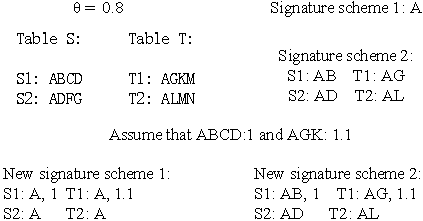
\includegraphics[scale=0.8]{figures/signature_example1}
% \caption{Illustration to the difference of signature schemes}
%\label{fig:signature_example1}
%\end{figure}
%
%A Count-Min (CM) sketch with parameters ( $\varepsilon, \delta$) is represented by a two-dimensional
%array counts with width $w$ and depth $d$. Given parameters ($\varepsilon, \delta$), set
%$w$ = $\lceil \frac{e}{\varepsilon} \rceil$ and $d$ = $\lceil ln \frac{1}{\delta} \rceil $. Each entry of the array is initially zero.
%
%
%When a data item ($w,i$) arrives, meaning that the signature $w$ has the length $i$, then $i$ is added to one cell in each row; the counter is determined by $h_j$. Formally, set $\forall 1 \leq j \leq d$, then count[j,$h_j(i)$]
%
%
%The space used by Count-Min sketches is the array of $wd$ counts, which takes $wd$ words, and $d$ hash
%functions, each of which can be stored using 2 words when using the pairwise functions described in [27].
%
%Estimation procedure. Our estimation for $S \bigodot T $ = $min_j S_j \bigodot T_j $
%
%
%\begin{theorem}
%With a probability 1- $\delta$, The upper bound and lower bound of Composite signature estimation is
% $S \bigodot T $ and  $S \bigodot T $ + $\varepsilon |S| |T|$, respectively.
%\end{theorem}
%
%\begin{theorem}
%Our composite signature estimation estimates the lower and upper bounds of algorithms by keeping space $O(\frac{1}{\varepsilon} \log \frac{1}{\delta})$ and
%\end{theorem}
%
%\subsubsection{Estimation with length filters}
%
%When we use the CountMin sketch to estimate the effectiveness of length filter. It is to



%\subsection{Extensions for flexible query thresholds} \label{subsec:flexible}
%
%In the previous sections, our model assumes that the search threshold is fixed, and only the query can be changed online. However, in practice users might change the threshold at query-time. Therefore, we now move to a more general case, where both the search string and the threshold are flexible at query-time. The new challenge here is that we do not know the threshold in advance and thus we cannot determine the number of signatures of each record. A na\"{i}ve method is to compute the signatures of records in the table online according to the given threshold, which  is clearly prohibitively expensive. Next we build a new index called \textit{FSI-trees} (Flexible Signature Indexing) by extending SI-trees to solve this problem.
%
%Suppose that all meaningful thresholds distribute in the range between 0.99 to 0.50. Then we select some \textit{representative thresholds}, e.g. 0.95, 0.90, etc.   For each representative threshold, we generate signatures for each record. See an example in Figure \ref{fig:FSI}(a). Note that the signatures of a string for lower thresholds are guaranteed to become signatures of that for higher thresholds. To build an FSI-tree,  the length and fence entries of SI-trees remain the same. But each fence entry points to a set of I-lists which come from \textit{all} representative thresholds. Further, each element in the I-list of a signature token $s$ is a binary tuple ($q$, $\theta$), where $q$ is a record ID and $\theta$ is the minimal threshold for which this signature $s$ appears in $q$. For example, in Figure \ref{fig:FSI}(b), the token ``\textsf{Computing}''  is a signature of $q_1$ for all thresholds $\geq 0.5$.
%
%We extend the QP-search algorithm for flexible thresholds. The algorithm almost remains the same, but  the only  change (See Algorithm \ref{algo:QP-flexible}) is that we select the string candidates in I-lists by checking their thresholds (Line 3).
%
%An astute reader may notice that our method possibly introduces more candidates because of the gap between representative thresholds and online thresholds. For example, given a query threshold 0.83, suppose that the closest representative threshold is 0.80. Then  the number of signatures for threshold 0.80  may be greater than that for 0.83. But we argue that the problem  has actually a little impact on the final performance of query processing. To understand this, assume that gap between two representative thresholds is no more than 0.05 (that means, only 11 representative thresholds are ``materialized'' with signatures between 0.99 and 0.50). It can be proved that given a string $s$, the difference between the numbers of signatures for thresholds $\theta_1$ and $\theta_2$ is $\lceil  |\theta_1 - \theta_2|   \cdot |s| \rceil$. Considering a string $|s|$=10, we have 0.05 * 10 =0.5, That is, for most records in the table, the extra number of signatures due to the thresholds gap  is bounded by 0.5. Therefore, as our experimental results show in Section \ref{subsec:searchalgorithms}, the performance of our algorithms for flexible thresholds is comparable to that for static thresholds.



